\documentclass[tikz,dvisvgm,border=0pt]{standalone}
% Shared preamble of the diagrams in vignettes/articles/cuda-kernels.Rmd.
% Render them with `make diagrams` from the package root.
\usepackage[T1]{fontenc}
\usepackage{lmodern}
\usepackage{tikz}
\usetikzlibrary{arrows.meta, positioning, fit, backgrounds, calc, shapes.geometric, decorations.pathreplacing}

\definecolor{host}{HTML}{3B6EA8}
\definecolor{device}{HTML}{2E8B57}
\definecolor{accent}{HTML}{C0571B}
\definecolor{muted}{HTML}{6B6B6B}

% A white card behind every figure, so that it reads in pkgdown's dark mode.
\tikzset{
  every picture/.append style={
    show background rectangle,
    background rectangle/.style={fill=white, rounded corners=6pt},
    inner frame sep=8pt,
    font=\sffamily\small,
    >={Stealth[length=2.2mm]},
  },
  box/.style={draw, rounded corners=3pt, thick, align=center, inner sep=5pt, fill=white},
  hostbox/.style={box, draw=host, fill=host!8},
  devbox/.style={box, draw=device, fill=device!8},
  accbox/.style={box, draw=accent, fill=accent!8},
  region/.style={draw=#1, rounded corners=6pt, thick, dashed, inner sep=8pt},
  heading/.style={font=\sffamily\bfseries\small, text=#1},
  note/.style={font=\sffamily\footnotesize, text=muted, align=center},
  flow/.style={->, thick},
  code/.style={font=\ttfamily\footnotesize},
}

\begin{document}
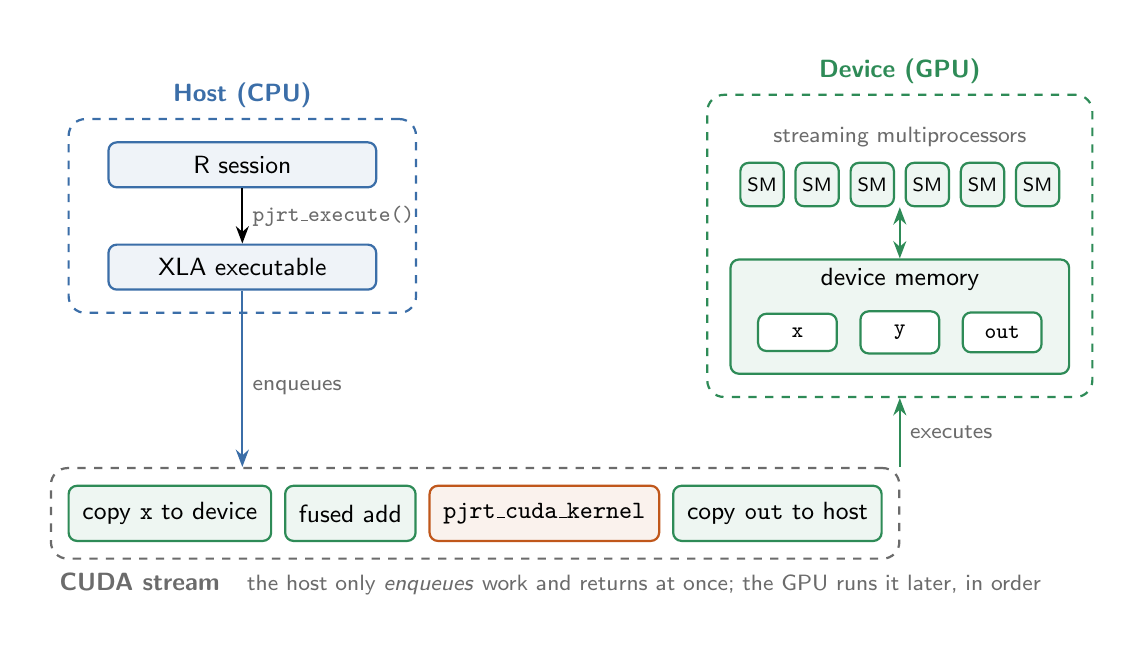
\begin{tikzpicture}
  % host
  \node[hostbox, minimum width=3.4cm] (r) at (0, 0) {R session};
  \node[hostbox, minimum width=3.4cm, below=0.7cm of r] (xla) {XLA executable};
  \draw[flow] (r) -- node[right, note] {\texttt{pjrt\_execute()}} (xla);
  \node[region=host, fit=(r)(xla), inner xsep=14pt, label={[heading=host]above:Host (CPU)}] (hostregion) {};

  % device
  \foreach \i in {0,...,5} {
    \node[devbox, minimum size=0.55cm, inner sep=0pt, font=\sffamily\scriptsize]
      (sm\i) at ({6.6 + 0.7*\i}, -0.25) {SM};
  }
  \node[note, above=2pt of $(sm2.north)!0.5!(sm3.north)$] (smlabel) {streaming multiprocessors};
  \node[devbox, minimum width=4.3cm, minimum height=1.45cm, anchor=north]
    (dmem) at ($(sm2.south)!0.5!(sm3.south) + (0, -0.65)$) {};
  \node[anchor=north, font=\sffamily\small] at (dmem.north) {device memory};
  \foreach \n/\x in {x/-1.3, y/0, out/1.3} {
    \node[box, draw=device, minimum width=1.0cm, font=\ttfamily\footnotesize] at ($(dmem.center) + (\x, -0.2)$) {\n};
  }
  \draw[<->, thick, device] ($(sm2.south)!0.5!(sm3.south)$) -- (dmem.north);
  \node[region=device, fit=(smlabel)(sm0)(sm5)(dmem), label={[heading=device]above:Device (GPU)}] (devregion) {};

  % the stream
  \node[devbox, minimum height=0.7cm, anchor=north west] (q1) at ($(hostregion.west |- devregion.south) + (0, -1.1)$) {copy \texttt{x} to device};
  \node[devbox, minimum height=0.7cm, right=0.15cm of q1] (q2) {fused add};
  \node[accbox, minimum height=0.7cm, right=0.15cm of q2] (q3) {\texttt{pjrt\_cuda\_kernel}};
  \node[devbox, minimum height=0.7cm, right=0.15cm of q3] (q4) {copy \texttt{out} to host};
  \node[region=muted, fit=(q1)(q4), inner sep=6pt] (stream) {};
  \node[heading=muted, anchor=north west] (streamlabel) at ($(stream.south west) + (0, -0.05)$) {CUDA stream};
  \node[note, anchor=base west] at ($(streamlabel.base east) + (0.1, 0)$)
    {the host only \emph{enqueues} work and returns at once; the GPU runs it later, in order};

  \draw[flow, host] (xla.south) -- (xla.south |- stream.north)
    node[pos=0.55, right, note] {enqueues};
  \draw[flow, device] (stream.north -| dmem.south) -- (devregion.south -| dmem.south)
    node[pos=0.5, right, note] {executes};
\end{tikzpicture}
\end{document}
